
En este capítulo, exploraremos las primeras técnicas utilizadas para representar el lenguaje en forma vectorial. Para contextualizar esto, planteamos las siguientes preguntas:

\begin{itemize}
   \item ¿Cómo recuperan los motores de búsqueda, como Duckduckgo o Google, los documentos relevantes a partir de una consulta dada?
   \item ¿Cómo pueden las empresas procesar las reclamaciones dejadas por sus usuarios en sus portales web?
\end{itemize}

Estas preguntas suelen abordarse desde dos disciplinas relacionadas:

\begin{itemize}
   \item \emph{Recuperación de Información}: ciencia que se ocupa de buscar información en colecciones de documentos.
   \item \emph{Minería de Texto}: extracción automática de conocimiento a partir de texto.
\end{itemize}

Ambas disciplinas están estrechamente vinculadas al PLN, y las fronteras entre estos campos no siempre están claras.

\section{Tokens y Tipos}

El primer paso en el procesamiento de texto es, generalmente, la \textbf{tokenización}, que consiste en dividir una oración o documento en fragmentos llamados \emph{tokens}. A menudo, se acompañan otras transformaciones adicionales, como la eliminación de caracteres especiales (por ejemplo, puntuación), la conversión de todo el texto a minúsculas y otras operaciones descritas en este capítulo.

\begin{example}
Entrada: ``Me gustan los lenguajes humanos y los lenguajes de programación.''

Tokens: [Me] [gustan] [los] [lenguajes] [humanos] [y] [los] [lenguajes] [de] [programación] 
\end{example}




\subsection{Tipos}

Un \emph{tipo} es una clase de \emph{token} que contiene una secuencia única de caracteres. Los tipos se obtienen identificando los tokens únicos dentro del documento.

\begin{example}
Por ejemplo, para la oración anterior, los tipos serían: [Me] [gustan] [los] [lenguajes] [humanos] [y] [de] [programación]. Observemos que el token \emph{lenguajes} se incluye solo una vez en la lista de tipos. 
\end{example}



\paragraph{Extracción de Vocabulario}

Un \emph{término} es un \emph{tipo} normalizado. La normalización implica la creación de clases de equivalencia para diferentes \emph{tipos}, por ejemplo, cuando tratamos de manera indistinta dos tokens que difieren solo en el uso de mayúsculas (hombre y Hombre). El vocabulario $V$ es el conjunto de términos (tokens únicos normalizados) dentro de una colección de documentos o corpus $D$.

\section{Eliminación de Stopwords}

Con el fin de reducir el tamaño del vocabulario y eliminar términos que no aportan mucha información, se eliminan los términos que ocurren con alta frecuencia en el corpus (o colección de documentos). Estos términos se llaman \emph{stopwords} e incluyen artículos, pronombres, preposiciones y conjunciones.

\begin{example}
Ejemplo de stopwords: [un, una, y, cualquier, no, el, en]. 
\end{example}


Es importante tener en cuenta que la eliminación de stopwords puede ser inconveniente en muchas tareas de procesamiento del lenguaje natural. 

\begin{example}
Por ejemplo, en la oración ``No me gusta la pizza'', al eliminar la negación, se pierde información valiosa sobre el sentimiento de la oración. 
\end{example}



\section{Stemming}

Es un proceso de normalización de términos en el cual los términos se transforman a su raíz con el objetivo de reducir el tamaño del vocabulario. Se lleva a cabo aplicando reglas de reducción de palabras. La Tabla~\ref{tab:porter} muestra  algunas reglas del algortimo de Porter para el inglés con ejemplos de aplicación:

\begin{table}[h]
\centering
\begin{tabular}{|l|l|}
\hline
Regla & Ejemplo \\
\hline
SSES $\rightarrow$ SS & caresses $\rightarrow$ caress \\
IES $\rightarrow$ I & ponies $\rightarrow$ poni \\
SS $\rightarrow$ SS & caress $\rightarrow$ caress \\
S $\rightarrow$ & cats $\rightarrow$ cat \\
\hline
\end{tabular}
\caption{Ejemplos del Algortimo de Porter}
\label{tab:porter}
\end{table}

\begin{example}

A continuación se muestra ejemplo usando el método de stemming Snowball para español para el lenguaje \textbf{python} usando la biblioteca \textbf{nltk}\footnote{\url{https://www.nltk.org/}}.

\begin{verbatim}
from nltk import word_tokenize
from nltk.stem import SnowballStemmer
stemmer = SnowballStemmer('spanish')
texto = 'Me gustan los lenguajes humanos y los lenguajes de programación'
def stem_sentence(text):
    return ' '.join([stemmer.stem(i) for i in word_tokenize(text)])    
print(stem_sentence(texto))
>>
me gust los lenguaj human y los lenguaj de program
\end{verbatim} 
\end{example}




\section{Lematización}
Otra estrategia de normalización de términos. También transforma las palabras en sus raíces.  Realiza un análisis morfológico utilizando diccionarios de referencia (tablas de búsqueda) para crear clases de equivalencia entre \emph{tipos}. Por ejemplo, para el token \emph{yendo}, una regla de stemming devolvería el término \emph{yend}, mientras que a través de la lematización obtendríamos el término \emph{ir}.

\begin{example}
Veamos a continuación el resultado de aplicar lematización a la misma oración anterior con la biblioteca \textbf{spacy}\footnote{\url{https://spacy.io/}}:

\begin{verbatim}
# python -m spacy download es_core_news_sm
import spacy
nlp = spacy.load('es_core_news_sm')

def lemmatizer(text):  
  doc = nlp(text)
  return ' '.join([word.lemma_ for word in doc])

print(lemmatizer(texto))
>>
yo gustar el lenguaje humano y el lenguaje de programación
\end{verbatim}
\end{example}





\section{Ley de Zipf}
La Ley de Zipf, propuesta por George Kingsley Zipf en \cite{zipf1935}, es una ley empírica que describe la frecuencia de los términos en una colección de documentos (corpus). Según esta ley, la frecuencia $f$ de un término en un corpus es inversamente proporcional a su posición $r$ en una tabla de frecuencias ordenada:

\begin{equation}
f = \frac{cf}{r^{\beta}}
\end{equation}

Aquí, $cf$ es una constante dependiente de la colección y $\beta > 0$ es un factor de decaimiento. Cuando $\beta = 1$, la frecuencia sigue exactamente la Ley de Zipf, de lo contrario, sigue una distribución similar a la de Zipf. Esta ley nos indica que algunas palabras se utilizan con mucha más frecuencia que otras en un corpus. La Ley de Zipf se clasifica como una distribución de ley de potencia, que es un tipo de distribución de cola larga.

\begin{figure}[h!]
\centering
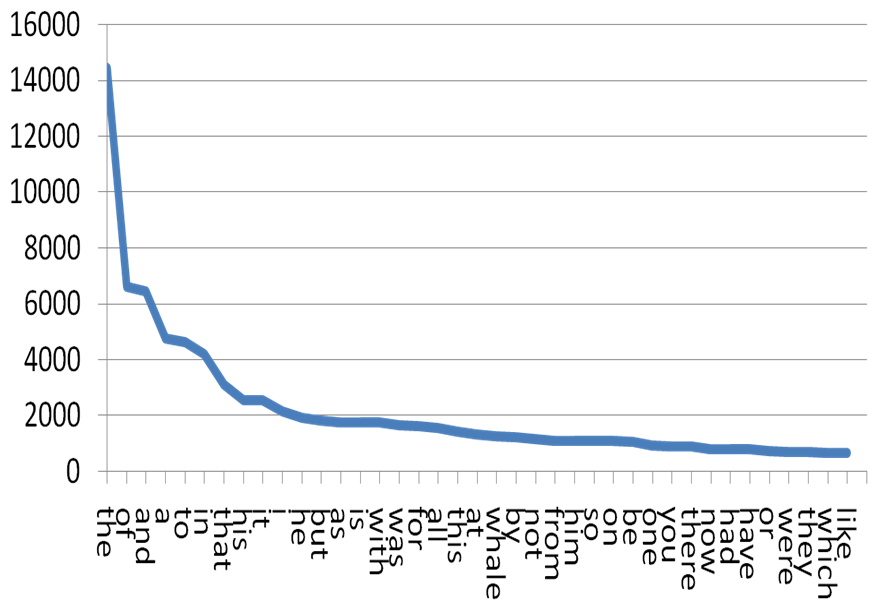
\includegraphics[scale=0.5]{pics/zipf1.png}
\caption{Ley de Zipf.}
\end{figure}

Cuando trazamos un gráfico en escala logarítmica ($log$-$log$), se obtiene una línea recta con una pendiente de $-\beta$. Esta relación logarítmica es útil para identificar las palabras más frecuentes en un corpus y construir una lista de stopwords.


\section{Listas de posteo y el índice invertido}
Sea $D$ una colección de documentos y $V$ el vocabulario de todos los términos extraídos de la colección:


\begin{definition}
La lista de posteo de un término es la lista de todos los documentos donde el término aparece al menos una vez. Los documentos se identifican por sus identificadores. 
\end{definition}

\begin{definition}
Un índice invertido es una estructura de datos tipo diccionario que mapea los términos $t_{i} \in V$ con sus listas de posteo correspondientes.
\begin{displaymath}
<\text{término}> \rightarrow <\text{idDocumento}>^*
\end{displaymath} 
\end{definition}



\begin{figure}[h!]
\centering
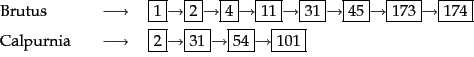
\includegraphics[scale=0.6]{pics/invFile.png}
\caption{Índice invertido}
\end{figure}

\section{Motores de búsqueda web}

Un motor de búsqueda es un sistema de recuperación de información diseñado para buscar información en la web (satisfacer necesidades de información) \cite{manning2008}. Sus componentes básicos (ilustrados en la Figura~\ref{fig_buscador}) son:

\begin{itemize}
\item Crawler: un robot que navega por la web según una estrategia definida. Por lo general, comienza navegando por un conjunto de sitios web iniciales (semillas) y continúa navegando a través de sus enlaces.
\item Indexador: se encarga de mantener un índice invertido con el contenido de las páginas recorridas por el crawler.
\item Procesador de consultas: se encarga de procesar las consultas de los usuarios y buscar en el índice los documentos más relevantes para una consulta.
\item Función de ranking: la función utilizada por el procesador de consultas para ordenar los documentos indexados en la colección por relevancia según una consulta.
\item Interfaz de usuario: recibe la consulta como entrada y devuelve los documentos ordenados por relevancia.
\end{itemize}


\begin{figure}[h!]
\centering
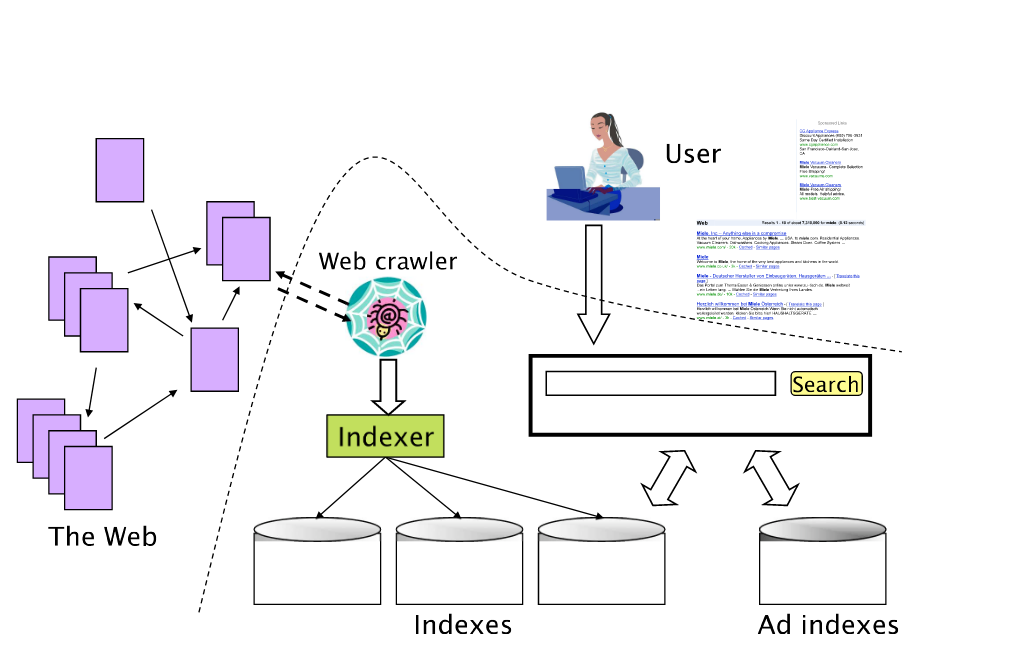
\includegraphics[scale=0.25]{pics/searchengine.png}
\caption{Los diversos componentes de un motor de búsqueda web \cite{manning2008}.}
\label{fig_buscador}
\end{figure}


\section{El modelo de espacio vectorial}
Para clasificar consultas o medir la similitud entre dos documentos, es esencial contar con una métrica que evalúe la similitud entre pares de documentos. Una estrategia para habilitar esta comparación implica la \textit{representación} de los documentos como vectores de términos, en la que cada término se convierte en una dimensión en el espacio vectorial \cite{salton1975vector}. De esta manera, documentos con diferentes palabras y longitudes pueden coexistir en el mismo espacio vectorial, lo que facilita su comparación. Estas representaciones se conocen como modelos de \emph{Bolsa-de-palabras} (Bag of Words), en los cuales se pierde información respecto al orden de las palabras y de la estructura lingüística de las oraciones, como se ilustra en la Figura~\ref{fig_bow}.


\begin{figure}[h!]
\centering
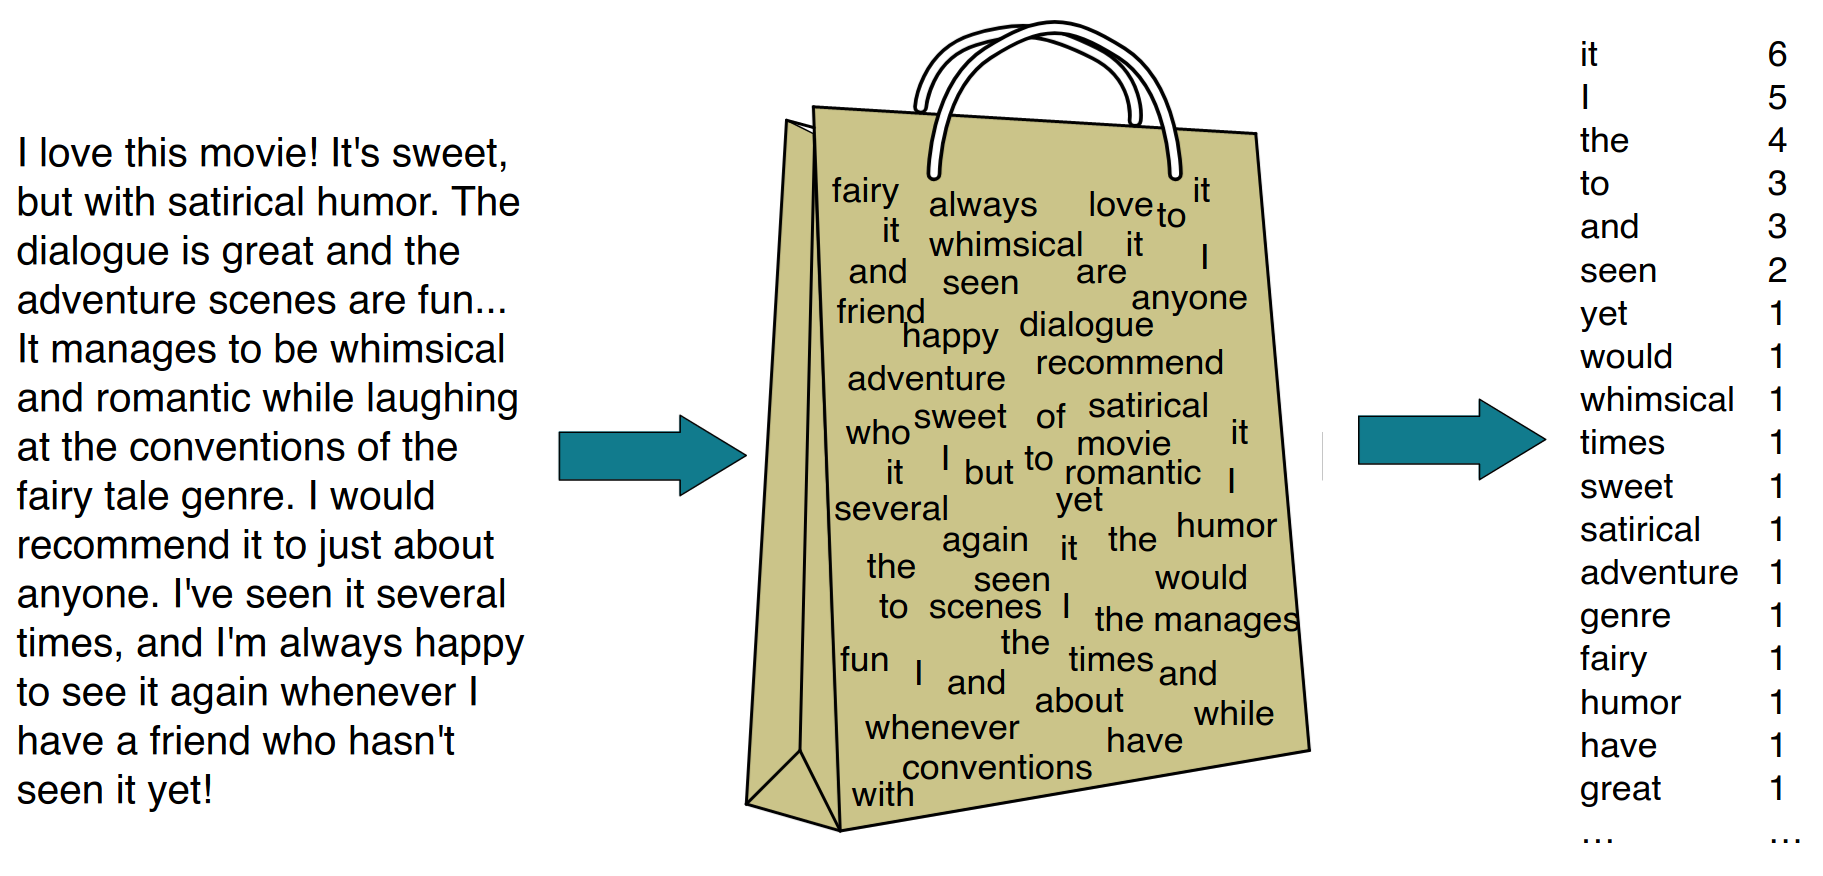
\includegraphics[scale = 0.22]{pics/bow.png}
\caption{Representación de Bolsa-de-Palabras \cite{JurafskyBook}.}
\label{fig_bow}
\end{figure}




El valor de cada dimensión es un peso que representa la relevancia del término $t_{i}$ en el documento $d$.
\begin{equation}
d_{j} \rightarrow \overrightarrow{d_{j}}=(w(t_{1},d_{j}),...,w(t_{|V|},d_{j}))
\end{equation}

Para cuantificar la importancia que un término aporta a un documento, es necesario emplear métodos de ponderación de su relevancia, denotada como $w(t_{i},d_{j})$. Una técnica ampliamente utilizada para abordar esto es el modelo de Frecuencia de Término - Frecuencia Inversa de Documento, comúnmente conocido como ``TF-IDF'' (por sus siglas en inglés).

\subsection{El modelo TF-IDF}
Definimos $tf_{i,j}$ como la frecuencia del término $t_{i}$ en el documento $d_{j}$. La lógica subyacente en esta ponderación es que un término que aparece 10 veces en un documento debería aportar más información que uno que solo aparece una vez. Sin embargo, surge un problema cuando tenemos documentos de diferentes longitudes, ya que no deseamos favorecer a los documentos más extensos. Para abordar esta cuestión, normalizamos la frecuencia dividiendo por la frecuencia máxima del término en el documento, como se muestra a continuación:

\[
ntf_{i,j} = \frac{tf_{i,j}}{\max_i (tf_{i,j})}
\]

Ahora podemos preguntarnos ¿un término que ocurre en muy pocos documentos proporciona más o menos información que uno que ocurre varias veces? Por ejemplo, el documento \emph{El respetado alcalde de Pelotillehue}. El término \emph{Pelotillehue} ocurre en menos documentos que el término \emph{alcalde}, por lo que debería ser más descriptivo. La frecuencia del término en el documento no es capaz de considerar esa relevancia. 

\begin{definition}
Sea $N$ el número de documentos en la colección y $n_{i}$ el número de documentos que contienen el término $t_{i}$, definimos la frecuencia inversa de documento ($idf$) de $t_{i}$ de la siguiente manera:
\begin{displaymath}
idf_{t_{i}}= \log_{10}\left(\frac{N}{n_{i}}\right)
\end{displaymath}

\end{definition}

Un término que aparece en todos los documentos tendría $idf=0$, y uno que aparece en el $10\%$ de los documentos tendría $idf=1$. 

\begin{definition}
 El modelo $tf$-$idf$ combina los valores de $tf$ e $idf$, y resulta en los siguientes pesos $w$ para un término en un documento:
\begin{displaymath}
w(t_{i},d_{j})=tf_{i}\times \log_{10}\left(\frac{N}{n_{i}}\right)
\end{displaymath} 
\end{definition}



Las consultas de los motores de búsqueda también pueden ser modeladas como vectores. Sin embargo, en promedio, las consultas suelen tener entre 2 y 3 términos. Para evitar tener demasiadas dimensiones nulas, los vectores de consulta pueden suavizarse de la siguiente manera:
\begin{displaymath}
w(t_{i},d_{j})=(0.5+0.5\times tf_{i,j})\log_{10}\left(\frac{N}{n_{i}}\right)
\end{displaymath}

\subsection{Similitud entre vectores}
Representar consultas y documentos como vectores permite calcular su similitud. Un enfoque podría ser utilizar la distancia euclidiana. El enfoque común es calcular el coseno del ángulo entre los dos vectores. Si ambos documentos son iguales, el ángulo sería $0$ y su coseno sería $1$. Por otro lado, si son ortogonales, el coseno es $0$. 

\begin{definition}
La similitud del coseno se calcula de la siguiente manera:
\begin{displaymath}
\text{similitud del coseno}(\vec{d}{1},\vec{d}{2})= \frac{\vec{d}{1}\cdot \vec{d}{2}}{|\vec{d}{1}|\times|\vec{d}{2}|} = \frac{\sum_{i=1}^{|V|}(w(t_{i},d_{1})\times w(t_{i},d_{2}))}{\sqrt{\sum_{i=1}^{|V|} w(t_{i},d_{1})^2}\times \sqrt{\sum_{i=1}^{|V|} w(t_{i},d_{2})^2}}
\end{displaymath} 
\end{definition}



Esto se llama incorrectamente ``distancia del coseno''. En realidad, es una métrica de similitud pues entre más cerca dos vectores mayor es el valor asociado. Nótese que la similitud del coseno normaliza los vectores por su norma euclidiana $||\vec{d}||_{2}$.

\begin{figure}[h!]
\centering
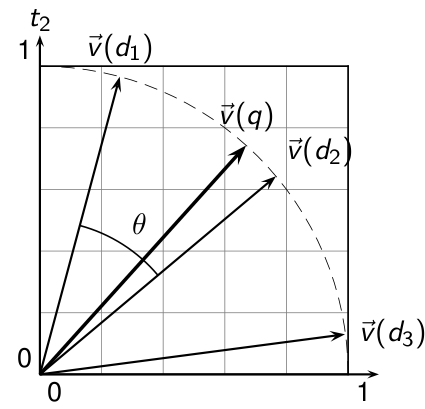
\includegraphics[scale=0.5]{pics/cos.png}
\caption{Similitud del coseno.}
\end{figure}

Un motor de búsqueda puede entonces usar el índice invertido para tener una representación vectorial de los documentos y así una vez llega una consulta usar la similitud coseno entre la consulta y los documentos indexados para producir el ranking de relevancia que se le muestra al usuario.

\paragraph{Ejercicio}
\begin{itemize}
\item Supongamos que tenemos $3$ documentos formados a partir de las siguientes secuencias de términos: \
$d_{1}\rightarrow t_{4}t_{3}t_{1}t_{4}$ \
$d_{2}\rightarrow t_{5}t_{4}t_{2}t_{3}t_{5}$ \
$d_{3}\rightarrow t_{2}t_{1}t_{4}t_{4}$ \
\item Construya una matriz término-documento de dimensiones $5\times3$ utilizando pesos simples de $tf$-$idf$ (sin normalización).
\item Recomendamos que primero construyas una lista con el número de documentos en los que aparece cada término (útil para calcular los valores de $idf$).
\item Luego, calcula los valores de $idf$ para cada término.
\item Rellena las celdas de la matriz con los valores de $tf$-$idf$.
\item ¿Cuál es el documento más cercano a $d_{1}$?
\end{itemize}

Resultado:
 \begin{table}[h]
 \centering
\begin{tabular}{|l|r|r|r|}
\hline
 & \multicolumn{1}{l|}{d1} & \multicolumn{1}{l|}{d2} & \multicolumn{1}{l|}{d3} \\ \hline
t1 & 0.176 & 0.000 & 0.176 \\ \hline
t2 & 0.000 & 0.176 & 0.176 \\ \hline
t3 & 0.176 & 0.176 & 0.000 \\ \hline
t4 & 0.000 & 0.000 & 0.000 \\ \hline
t5 & 0.000 & 0.954 & 0.000 \\ \hline
\end{tabular}
\caption{Matriz tf-idf}
\end{table}
\section{Clustering de Documentos}

¿Cómo podemos agrupar (o clusterizar) documentos que sean similares entre sí? El clustering es el proceso de agrupar documentos que comparten similitudes. Cada grupo de documentos se denomina \emph{cluster}. En el clustering, buscamos identificar grupos de documentos donde la similitud entre los documentos del mismo grupo se maximice, mientras que la similitud entre los documentos de diferentes grupos se minimice.

\begin{figure}[h!]
\centering
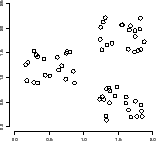
\includegraphics[scale=0.6]{pics/cluster.png}
\caption{Conjunto de documentos donde los grupos se pueden identificar claramente.}
\end{figure}

El clustering de documentos permite identificar tópicos en un corpus y reducir el espacio de búsqueda en un motor de búsqueda. Por ejemplo, el índice invertido se organiza según los grupos. El algoritmo K-means es una técnica de clustering simple que toma como parámetro el número de grupos, $k$.

El algoritmo se basa en la noción de \emph{centroides}, que son los vectores promedio de los documentos pertenecientes al mismo grupo. Por ejemplo, dado un conjunto de vectores bidimensionales $S = \{(3,6), (1,2), (5,1)\}$, el centroide de $S$ sería $(3,3)$, calculado como $(3+1+5)/3$ y $(6+2+1)/3$.

El algoritmo K-means comienza seleccionando $k$ centroides de manera aleatoria. Luego, calcula la similitud entre cada documento y cada centroide, asignando cada documento al centroide más cercano, formando así un grupo. Los centroides se recalculan de acuerdo con los documentos asignados a ellos. Este proceso se repite hasta que se cumple un criterio de convergencia, como se ilustra en el Algoritmo~\ref{algo:kmeans}.

\begin{algorithm}[H]
\SetKwInOut{Input}{Input}
\SetKwInOut{Output}{Output}
    \Input{Datos vectoriales $\vec{x}_1, \ldots, \vec{x}_N$ y el número de clusters $K$}
    \Output{centroides de clusters $\vec{\mu}_1, \ldots, \vec{\mu}_K$}
    $(\vec{s}_1, \vec{s}_2, \ldots, \vec{s}_K) \leftarrow$ SELECT\_RANDOM\_SEEDS($\vec{x}_1, \ldots, \vec{x}_N$, $K$)\;
    \For{$k \leftarrow 1$ \KwTo $K$}{
        $\vec{\mu}_k \leftarrow \vec{s}_k$\;
    }
    \While{no se cumpla el criterio de parada}{
        \For{$k \leftarrow 1$ \KwTo $K$}{
            $\omega_k \leftarrow \{\}$\;
        }
        \For{$n \leftarrow 1$ \KwTo $N$}{
            $j \leftarrow \arg\max_{j'} $coseno$(\vec{\mu}_{j'}, \vec{x}_n)$\;
            $\omega_j \leftarrow \omega_j \cup \{\vec{x}_n\}$\;
        }
        \For{$k \leftarrow 1$ \KwTo $K$}{
            $\vec{\mu}_k \leftarrow \frac{1}{{|\omega_k|}} \sum_{\vec{x} \in \omega_k} \vec{x}´$\;
        }
    }
    \Return{$\{\vec{\mu}_1, \ldots, \vec{\mu}_K\}$}\;
    \caption{K-Means}\label{algo:kmeans}
\end{algorithm}

\section{Modelos de Tópicos}
Otra familia de modelos valiosos para explorar colecciones de documentos son los modelos de tópicos, como Latent Dirichlet Allocation (LDA) \cite{blei2003latent}. Estos modelos asumen que cada documento es una mezcla de variables latentes llamadas tópicos, donde cada tópico es una bolsa de palabras con una probabilidad asociada.

LDA es uno de los modelos de tópicos más ampliamente utilizados y se basa en las siguientes suposiciones:

\begin{enumerate}
 \item Cada documento está compuesto por combinación probabilística de $K$ tópicos. La distribución de tópicos en un documento se puede representar mediante una distribución de probabilidad.

\item Cada tópico es una distribución probabílistica de palabras. Esto significa que cada palabra en un documento proviene de uno de los tópicos presentes en el documento.

\item La generación de palabras en un documento sigue un proceso de generación conjunta condicionado a la distribución de tópicos en el documento. Es decir, primero se selecciona un tópico de la distribución de tópicos del documento y luego se selecciona una palabra del tópico seleccionado.
\end{enumerate}


La inferencia en LDA a partir de un corpus de documentos se realiza utilizando técnicas de inferencia Bayesiana, como el Muestreo de Gibbs y la Inferencia Variacional. Describir más formalmente LDA se escapa del alcance de este apunte, por ahora podemos decir que se relaciona estrechamente a los Modelos de Lenguage Probablísticos a estudiar en el Capítulo~\ref{cap_plm}.

Si comparamos LDA con clusterizar documentos usando K-means, podemos decir que los tópicos que encuentra LDA puedan ser más fácilmente interpretados que los clusters obtenidos este último. Como cada tópico es una distribución de probabilidad sobre todas las palabras del corpus de entrenamiento, uno puede analizar las primeras 10, 15 o 30 palabras más probables de cada tópico para darle una interpretación. Análogamente uno puede analizar los tópicos más probables asignados a cada documento para entender los tópicos que trata. 

La Tabla~\ref{tab:lda} muestra cuatro tópicos identificados por LDA en su trabajo original \cite{blei2003latent} usando un corpus de resúmenes de artículos científicos. Se muestran las 15 palabras más probables para 4 tópicos identificados.

\begin{table}[h]
\centering
\begin{tabular}{|c|c|c|c|}
\hline
Arts & Budgets & Children & Education \\
\hline
NEW & MILLION & CHILDREN & SCHOOL \\
FILM & TAX & WOMEN & STUDENTS \\
SHOW & PROGRAM & PEOPLE & SCHOOLS \\
MUSIC & BUDGET & CHILD & EDUCATION \\
MOVIE & BILLION & YEARS & TEACHERS \\
PLAY & FEDERAL & FAMILIES & HIGH \\
MUSICAL & YEAR & WORK & PUBLIC \\
BEST & SPENDING & PARENTS & TEACHER \\
ACTOR & NEW & SAYS & BENNETT \\
FIRST & STATE & FAMILY & MANIGAT \\
YORK & PLAN & WELFARE & NAMPHY \\
OPERA & MONEY & MEN & STATE \\
THEATER & PROGRAMS & PERCENT & PRESIDENT \\
ACTRESS & GOVERNMENT & CARE & ELEMENTARY \\
LOVE & CONGRESS & LIFE & HAITI \\
\hline
\end{tabular}
\caption{Ejemplo de 4 tópicos y sus 15 palabras más probables.}
\label{tab:lda}
\end{table}

\section{Conclusiones y Conceptos Adicionales}

En este capítulo, hemos explorado la representación de documentos como vectores para calcular similitudes entre ellos. Los vectores de ``bolsa-de-palabras'' son una forma común de representar documentos, pero tienen limitaciones ya que carecen de estructura lingüística y pueden ser de alta dimensionalidad y dispersos.

Una alternativa para capturar expresiones de múltiples palabras es utilizar n-gramas de palabras, que son secuencias contiguas de $n$ palabras. Por ejemplo, representar ``New York'' como ``new\_york'' nos permite capturar la relación entre esas dos palabras en lugar de tratarlas como entidades separadas.

Es importante señalar que los sistemas modernos de recuperación de información van más allá de la similitud de vectores. Utilizan algoritmos como PageRank \cite{page1998pagerank} para determinar la relevancia de un sitio web basándose en los enlaces que lo apuntan. También emplean técnicas de aprendizaje automático que utilizan registros de consultas anteriores para mejorar el ranking de resultados. Además, el uso de grafos de conocimiento enriquece aún más los resultados al proporcionar información estructurada y relaciones entre entidades.

Es importante destacar que disciplinas como la recuperación de información y la minería de textos se centran menos en la estructura lingüística que PLN y más en producir algoritmos rápidos y escalables para procesar grandes volúmenes de texto.
